\begin{titlepage}
  \begin{center}

  {\Huge PISO}

  \vspace{25mm}

  \includegraphics[width=0.90\textwidth,height=\textheight,keepaspectratio]{img/AFRL.png}

  \vspace{25mm}

  \today

  \vspace{15mm}

  {\Large Jay Convertino}

  \end{center}
\end{titlepage}

\tableofcontents

\newpage

\section{Usage}

\subsection{Introduction}

\par
This core converts the parallel data into serial data. This is done on a positive clock edge in relation to the enable.
The enable sets the rate and should only be held high for the same period as the main clock.
\subsection{Dependencies}

\par
The following are the dependencies of the cores.

\begin{itemize}
  \item fusesoc 2.X
  \item iverilog (simulation)
  \item cocotb (simulation)
\end{itemize}

\input{src/fusesoc/depend_fusesoc_info.tex}

\subsection{In a Project}
\par
This core is made to interface for parallel to serial data. Data is loaded into the core, and then enable is pulsed to
push data out in a serial fashion. There is a count output that tells how many bits have been output. Data is always
presented at the output so when count is at 31, the serial data output has bit 31 presented at the output.
The series of steps to use it are as follows.
\begin{enumerate}
  \item Set pdata to input data, and set load to 1 (data will be loaded on positive clock edge to internal registers).
  \item Set load to 0.
  \item Pulse enable to 1 that is synced to the main clock. Only hold high for one period of the master clock.
  \item Repeat enable pulse untill dcount is equal to 0.
\end{enumerate}

\begin{lstlisting}[language=Verilog]
\end{lstlisting}

\section{Architecture}
\par
The only module is the piso module. It is listed below.

\begin{itemize}
  \item \textbf{piso} Convert parallel data to serial data. (see core for documentation).
\end{itemize}

Please see \ref{Module Documentation} for more information.

\subsection{Waveform}

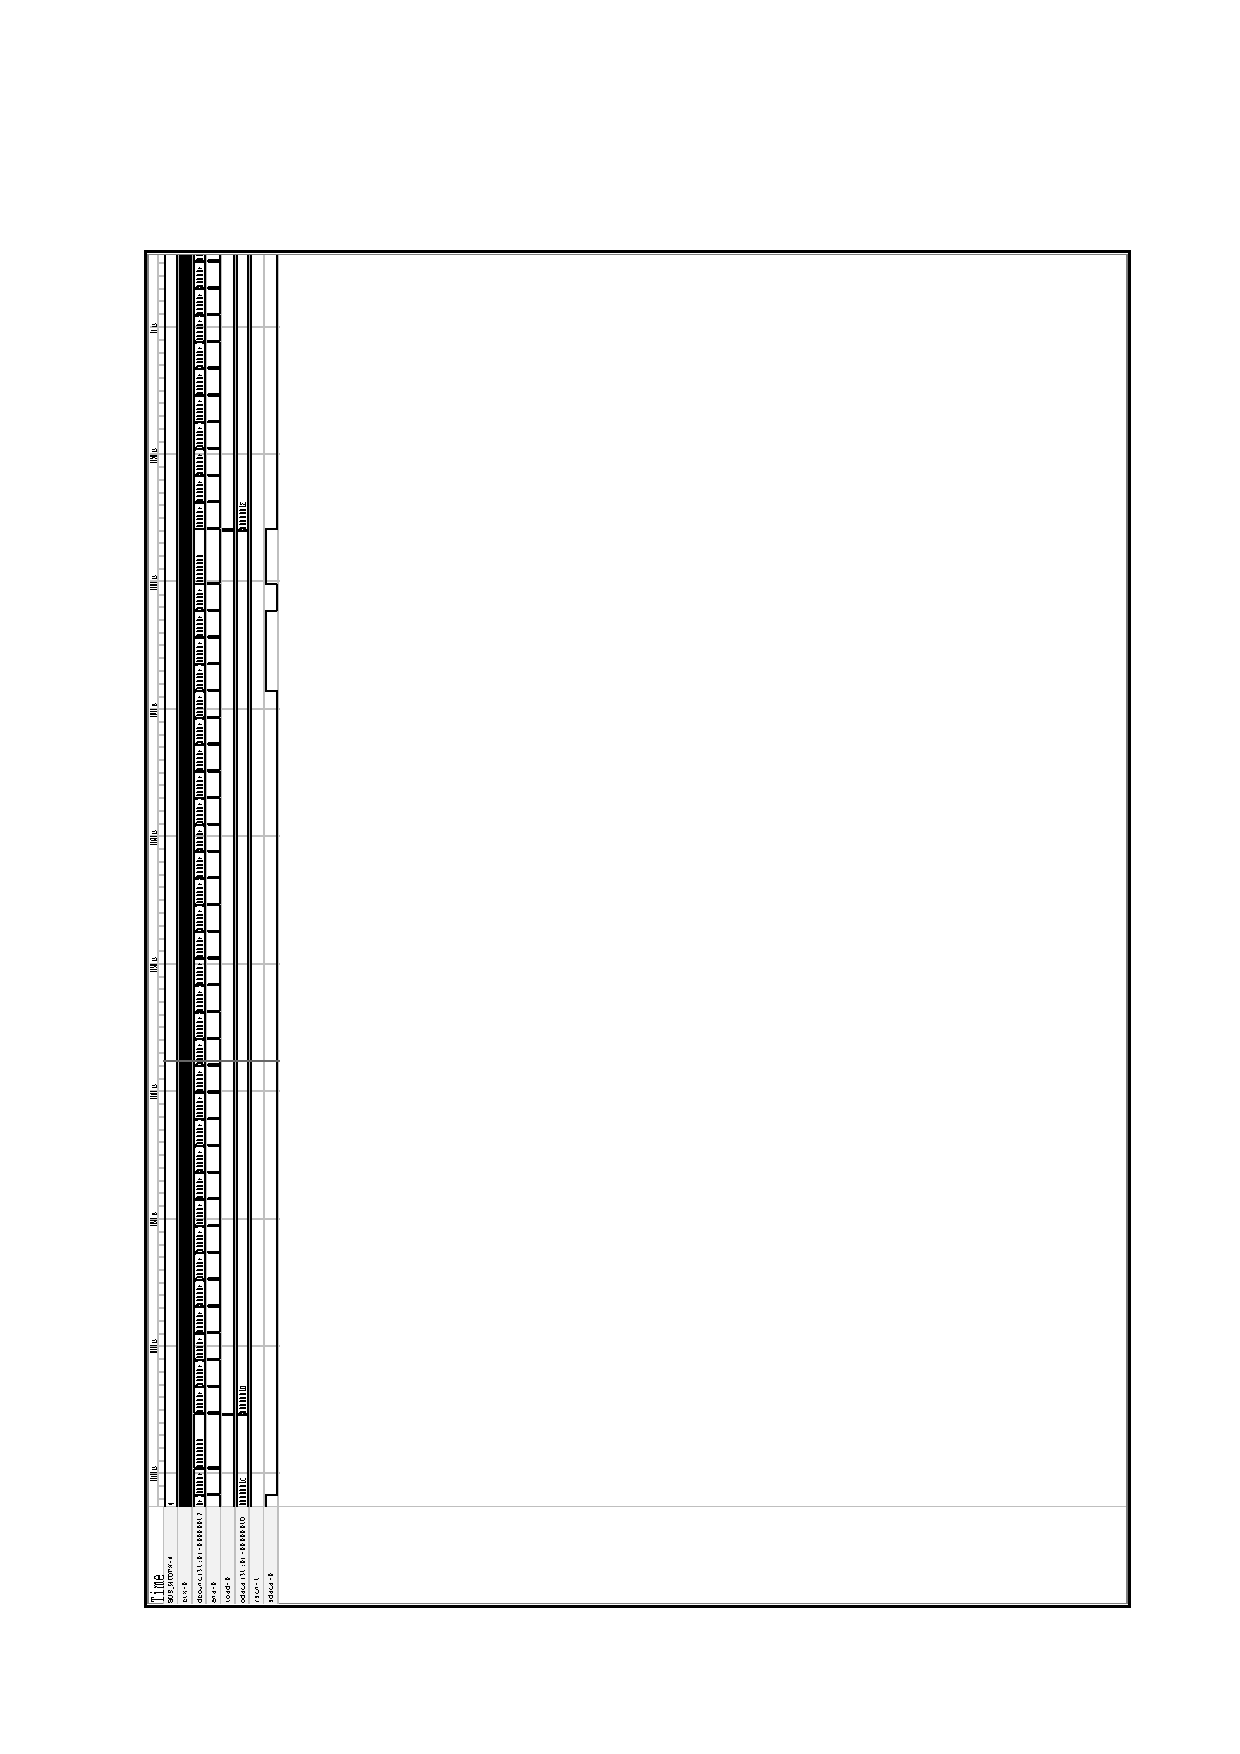
\includegraphics[width=\textwidth]{src/diagrams/waveform.png}

\section{Building}

\par
The PISO core is written in Verilog 2001. They should synthesize in any modern FPGA software. The core comes as a fusesoc packaged core and can be
included in any other core. Be sure to make sure you have meet the dependencies listed in the previous section.

\subsection{fusesoc}
\par
Fusesoc is a system for building FPGA software without relying on the internal project management of the tool. Avoiding vendor lock in to Vivado or Quartus.
These cores, when included in a project, can be easily integrated and targets created based upon the end developer needs. The core by itself is not a part of
a system and should be integrated into a fusesoc based system. Simulations are setup to use fusesoc and are a part of its targets.

\subsection{Source Files}

\input{src/fusesoc/files_fusesoc_info.tex}

\subsection{Targets}

\input{src/fusesoc/targets_fusesoc_info.tex}

\subsection{Directory Guide}

\par
Below highlights important folders from the root of the directory.

\begin{enumerate}
  \item \textbf{docs} Contains all documentation related to this project.
    \begin{itemize}
      \item \textbf{manual} Contains user manual and github page that are generated from the latex sources.
    \end{itemize}
  \item \textbf{src} Contains source files for the core
  \item \textbf{tb} Contains test bench files for iverilog and cocotb
    \begin{itemize}
      \item \textbf{cocotb} testbench files
    \end{itemize}
\end{enumerate}

\newpage

\section{Simulation}
\par
There are a few different simulations that can be run for this core.

\subsection{iverilog}
\par
iverilog is used for simple test benches for quick verification, visually, of the core.

\subsection{cocotb}
\par
To use the cocotb tests you must install the following python libraries.
\begin{lstlisting}[language=bash]
  $ pip install cocotb
\end{lstlisting}

\begin{itemize}
  \item \textbf{sim\_cocotb} Standard simulation PISO conversion using cocotb.
\end{itemize}

Then you must use the cocotb sim target. The targets above can be run with various parameters.
This test will check the input/output against each other to validate core operation.
\begin{lstlisting}[language=bash]
  $ fusesoc run --target sim_cocotb AFRL:simple:piso:1.0.0
\end{lstlisting}

\newpage

\section{Module Documentation} \label{Module Documentation}

\par

\begin{itemize}
\item \textbf{piso} PISO converter\\
\item \textbf{tb\_piso-v} Verilog test bench\\
\item \textbf{tb\_cocotb-py} Cocotb python test routines\\
\item \textbf{tb\_cocotb-v} Cocotb verilog test bench\\
\end{itemize}
The next sections document the module in detail.

